\chapter{Méthode de Gauss pour les systèmes linéaires et factorisation LU}
\chaptermark{Gauss pour systèmes linéaires et factorisation LU}

Soit $A \in M_n(\R)$ inversible et $b \in \R^n$. La méthode de Gauss permet de résoudre le système $Ax=b$, $x \in \R^n$ en se ramenant à la résolution d'un système triangulaire.
Nous allons commencer par rappeler cette méthode classique de résolution des systèmes linéaires. Il s'agit d'une \underline{méthode directe}, càd qui donne la solution exacte un nombre fini d'opérations arithmétiques élémentaires.
Nous verrons ensuite que l'élimination de Gauss fournit une factorisation $A = LU$ (ou $PA = LU$, $P$ étant une matrice de permutation, dépendant du choix des pivots)
avec $L$ triangulaire inférieure et $U$ triangulaire supérieure.
Résoudre $Ax=b \Leftrightarrow PAx = Pb \Leftrightarrow LUx = Pb$ revient donc à :

\begin{enumerate}
    \item Factoriser $PA$
    \item Résoudre $Lc = Pb$ (étape de \underline{descente}) $c_1 \to c_2 \to \dots \to c_n$
    \item Résoudre $Ux = c$ (étape de \underline{remontée}) : $x_n \to x_{n-1} \to \dots \to x_1$
\end{enumerate}

Si on doit résoudre de nombreuses fois avec la même matrice :
\[
    Ax^{(k)}=b^{(k)}
\]

Schémas ``implicites'' pour des EDP, schémas itératifs pour des systèmes linéaires ou non linéaires, \dots) alors l'étape 1) qui est la plus coûteuse est effectuée une seule fois.



\section{Rappel de l'élimination de Gauss :}

Soit $A \in M_n(\R)$ inversible et $b \in \R^n$. On cherche $x \in \R^n$ tel que $Ax=b$, soit :

\begin{equation}
    \left\lbrace
    \begin{array}{ccc}
        a_{11}X_1 + a_{12}X_2+ \dots+ a_{1n}X_n & = & b_1 \\
        \vdots \\
        a_{n1}X_1 + a_{n2}X_2 + \dots + a_{nn}X_n & = & b_n
    \end{array}\right.
\end{equation}


En notant $L_i = (a_{i1}, \cdots, a_{in})$ la i\up{ème} ligne de $A$, on a
\begin{equation}
    \left\lbrace
    \begin{array}{ccc}
        L_1 X = b_1 \\
        \vdots \\
        L_n X = b_n
    \end{array}\right.
    \tag{S}
    \label{eq:S}
\end{equation}


Si $a_{11} \neq 0$, on peut éliminer la variable $x_1$ dans les lignes 2 à $n$. On dit qu'on choisit $a_{11}$ comme \underline{pivot}.
$(S)$ équivaut à :
\[
    \left\lbrace
    \begin{array}{ccc}
        L_{1}X & = & b_1 \\
        (L_i - \frac{a_{i1}}{a_{11}}L_1) X & = & b_i - \frac{a_{i1}}{a_{11}}b_1 
    \end{array}\right.
    \hspace{2cm} i = 2..n
\]

Le nouveau système s'écrit $A^{(2)}X =b^{(2)}$ avec

\[
    A = 
    \begin{pmatrix}
        a_{11}^{(1)} & \cdots & a_{1n}^{(1)} \\
        0 \\
        \vdots \\
        0
    \end{pmatrix} 
    ,
    (a_{ij}^{(1)} = a_{ij})
\]

Ligne $i = L_i - l_{i1}L_1$ avec $l_{i1} = \frac{a_{i1}}{a_{11}}$

$b_i^{(2)} =  b_i - l_{i1}b_1$

Si $a_{11}$ on permute la 1ère ligne de \reff{eq:S} avec une autre ou $a_{i1} \neq 0$. Cela est toujours possible puisque $A$ est inversible.
On effectue la même procédure que précédemment expliqué.

Le système $A^{(2)} X = b^{(2)}$ contient un sous-système de dimension $n-1$ pour $x_2\dots x_n$
On répète la même procédure sur le sous-système pour éliminer $X_2$ des lignes 3 à $n$.

On continue ainsi et on déduit
\[
    A^{(3)}X = b^{(3)}, A^{(4)}X = b^{(4)}, \dots, A^{(n)}X=b^{(n)}
\]
Le dernier système obtenu est triangulaire. Notons $A^{(n)}=U$, $b^{(n)}=C$.

\begin{equation}
    \left\lbrace
    \begin{array}{ccccccc}
        u_{11}x_1 & + & \dots & + & u_{1n}x_n & = & c_1 \\
                  & u_{22}x_2 + & \dots & + & u_{2n}x_n & = & c_2 \\
        & & & \ddots \\
        & & & & u_{nn}x_n & = & c_n \\
    \end{array}\right.
    \tag{S'}
    \label{eq:S2}
\end{equation}

\reff{eq:S2} est facile à résoudre : \underline{``étape de remontée''}.
\[
    x_{nn} = \frac{c_n}{u_{nn}}, x_i = \frac{1}{u_{ii}}(c_i - \sum_{j=i+1}^{n}u_{ij}x_j )
\] pour $i = n-1, \dots, 1$

\begin{remark}
    On appelle \underline{``factorisation''} le calcul de $U$.
\end{remark}









\section{Factorisation LU}
Nous avons vu que l'élimination de Gauss peut conduire à permuter des lignes de A puisqu'on a besoin de ``pivots'' non nuls $a_{11}^{(1)}, a_{22}^{(2)}$ etc \dots Les cas où ces pivots sont voisins de 0 conduisent à des problèmes numériques (voir plus loin). Il est donc fréquent d'effectuer des permutations des lignes de A lors de l'élimination de Gauss.
Nous allons tout d'abord voir que ces permutations sont une traduction matricielle simple.

Notons ${p_1,p_2,\dots,p_n}$ une permutation des entiers ${1,2,\dots,n}$ et $(e_1,\dots,e_n)$ la base canonique de $\R^n$. On appelle \underline{matrice de permutation} une matrice de la forme :

\[
    P =
    \begin{pmatrix}[c|c|c|c]
        e_{p_1} & e_{p_2} & \dots & e_{p_n}\\
\end{pmatrix} 
\]

On a $p_{l_i} = e_{p_i}$ et :

\[
    P
    \begin{pmatrix}
        x_1 \\ x_2 \\ \vdots \\ x_n
    \end{pmatrix}
    =
    \begin{pmatrix}
        \vdots \\ \vdots \\ x_j \\ \vdots
    \end{pmatrix}
    \text{$\leftarrow$ ligne $p_j$}, \hspace{1cm}
    P
    \underbrace{\begin{pmatrix}
        L_1 \\
        L_2 \\
        \vdots \\
        L_n
    \end{pmatrix}
    }_\text{A}
    =
    \begin{pmatrix}
        \vdots \\
        \vdots \\
        L_j \\ 
        \vdots
    \end{pmatrix}
    \text{$\leftarrow$ ligne $p_j$}
\]

Soit $A \in M_n(\R)$. Notons $P$ la matrice correspondant aux permutations effectuées sur les lignes de $A$ dans l'algorithme du paragraphe \textbf{1}.
On a donc $PA = \tilde{A}$, où l'élimination de Gauss sur $\tilde{A}$ se fait sans permutation. Le passage de $A^{(j-1)}$ à $A^{(j)}$ s'écrit (même notations qu'auparavant) : 
\[
    \text{Ligne $i$} = L_i - L_j \times \left( \frac{a^{(j-1)}_{ij}}{a^{(j-1)}_{jj}} \right), \hspace{0.5cm} i = j+1, \dots , n
\]

Soit matriciellement :
\[
    A^{(j)} = T_j A^{(j-1)}, \hspace{0.5cm} T_j =
    \begin{pmatrix}[c|c]
        \begin{matrix}[ccc]
        & & \\
        & I_j & \\
        & & \\
        \end{matrix} 
        &
        \begin{matrix}
            \scalebox{1.5}{0}
        \end{matrix}
        \\ \hline
        \begin{matrix}[ccc|c]
            & & & -l_{j+1,j} \\
            & \scalebox{1.5}{0} & & \vdots \\
            & & & -l_{n,j}
        \end{matrix}
        &
        \begin{matrix}[ccc]
        & & \\
        & I_{n_j} & \\
        & & \\
        \end{matrix} 
    \end{pmatrix}
\]

\[
    l_{ij} = \frac{a^{(j-1)}_{ij}}{a^{(j-1)}_{jj}} , \hspace{0.5cm} I_k = \text{matrice identité de taille $k$}
\]

    En effet : 
\[
    \begin{blockarray}{cccc}
        \begin{block}{c(ccc)}
            & & 0 & \\
            \cline{2-4}
            & & 0 & \\
            \cline{2-4}
            \text{\scalebox{0.7}{ligne $i \rightarrow$}} & 0 \dots 0 & 1 & 0 \dots 0 \\
            \cline{2-4}
            & & 0 & \\
            \cline{2-4}
            & & 0 & \\
        \end{block}
        & & \text{\scalebox{0.7}{$\uparrow$ colonne $j$}} & & \\
    \end{blockarray}
    \times
    \begin{pmatrix}
        L_1 \\ \hline
        L_2 \\ \hline
        \vdots \\ \hline
        L_n
    \end{pmatrix}
    =
    \begin{pmatrix}
        0 \\ \hline
        0 \\ \hline
        L_j \\ \hline
        0 \\ \hline
        0
    \end{pmatrix} \text{$\leftarrow$ ligne $j$}
\]

On a donc :
\[
    U = A^{(n-1)} = T_{n-1} \times T_{n-2} \times \dots \times T_1 \times PA = TPA
\]
Avec $U$ triangulaire supérieure et $T$ triangulaire inférieure (produit de matrices triangulaires inférieures).

Donc on a $PA=LU$ avec $L=T^{-1}$ triangulaire inférieure (l'inverse d'une matrice triangulaire inférieure l'est aussi).

\begin{remark}
    Dans $\ref{eq:S2}$ on a $C=TPb$ et donc $LC=Pb$.
\end{remark}

% l_ij à afficher en plus grand ... 
Soit maintenant :\[
    \tilde{L} =
    \begin{pmatrix}
        1 & & \scalebox{1.2}{0} \\
        & \ddots & \\
        l_{ij} & & 1
    \end{pmatrix}
\]

On a : 
\[
    T_1 \tilde{L} =
    \begin{pmatrix}
        1      &        &        & 0 \\
        0      & 1      &        &   \\
        \vdots &        & \ddots &   \\
        0      & l_{ij} &        & 1
    \end{pmatrix}
    , \dots , T_{n-1} \times T_{n-2} \times T_1 \tilde{L} = I
\]

Donc $L = \tilde{L}$. Nous avons donc montré le résultat suivant :

\begin{ftheo}[Factorisation LU d'une matrice inversible]
    Soit $A \in M_n(\R)$ inversible. Il existe une matrice de permutation $P$
et deux matrices triangulaires L (triangulaire inférieure de diagonale unité) et $U$ (triangulaire supérieure inversible) telles que $PA = LU$.

    Cette décomposition est donnée explicitement par l'élimination de Gauss, avec 
    (les coefficients $l_{ij}$ sont ceux de l'élimination de Gauss sur $\tilde{A}$) :

    \[
        L = \begin{pmatrix}
            1 & & 0 \\
            & \ddots & \\
            l_{ij} & & 1 \\
        \end{pmatrix}
        , U =
        \begin{pmatrix}
            \ddots & & U_{ij} \\
            & \ddots & & \\
            0 & &
        \end{pmatrix}
    \]

    Cette factorisation est unique lorsque l'on fixe P.
    \label{th:factoLU}
\end{ftheo}

\begin{remark}
    L'unicité s'obtient simplement :
    $PA$ est inversible (puisque $P$ et $A$ le sont).

    Si $PA = L_1 U_1 = L_2 U_2$ alors $L_i$ et $U_i$ sont inversibles et donc
    $L^{-1}_2 L_1 = U_2 U^{-1}_1$. Le membre de droite est triangulaire supérieur, celui de gauche et triangulaire inférieur de diagonale unité.

    Donc $L^{-1}_2 L_1 = U_2 U^{-1}_1 = I$, i.e. $L1 = L2$ et $U_1 = U_2$.
\end{remark}

\vspace{0.7cm}
Les permutations effectuées lors de l'élimination de Gauss sont très importantes d'un point de vue numérique (voir plus loin).
Bien sûr, si l'on raisonne en arithmétique exacte (sans tenir compte des erreurs d'arrondi)
on voit dans l'algorithme de Gauss que les cas nécessiteant une permutation sont
exceptionnels (cela se produit lorsque $a_{11}$ ou $a^{(i)}_{i+1,i+1}=0$ pour certaines valeurs de $i$).

On a plus précisément le résultat suivant :

\begin{ftheo}
    Dans le théorème \ref{th:factoLU}, si les $n$ sous-matrices
    \[\Delta = \begin{pmatrix}
        a_{11} & \dots & a_{1i} \\
        \vdots & & \vdots \\
        a_{i1} & \dots & a_{ii}
    \end{pmatrix}
, (1 \leq i \leq n)\]
    sont inversibles, alors on peut fixer $P = I$.
\end{ftheo}

\begin{preuve}
    $a_{11} \ne 0$ donc la 1\up{ère} de l'élimination de Gauss ne nécessite pas de permutation.
    Supposons qu'on ait $j$ étapes sans permutation :
    \[
        A^{(j)} =
        \begin{pmatrix}[c|c]
            U^{(j)} & X \\ \hline
            0 & X
        \end{pmatrix}
        = T_j T_{j-1} \times \dots \times T_1 \times A =
        \begin{pmatrix}[c|c]
            \begin{matrix}
                1 & & 0 \\
                & \ddots & \\
                X & & 1
            \end{matrix}
            & \begin{matrix}[ccc]\\ & 0 & \\ \end{matrix}
            \\ \hline
            \begin{matrix}[ccc]\\ & X & \\ \end{matrix}
            & \begin{matrix}[ccc]\\ & I & \\ \end{matrix}
        \end{pmatrix}
        \begin{bigmatrix}{2.5}{c|c}
            \Delta_j & X \\
            \hline
            X & X
        \end{bigmatrix}
    \]
    avec $U^{(j)} \in M_j(\R)$ de la forme 
    $\begin{pmatrix} 
        a_{11} & & & X \\
        & a_{22}^{(1)} & & \\
        & & \ddots & \\
        0 & & & a_{jj}^{(j)}
    \end{pmatrix}$
    (les coefficients diagonaux sont les pivots).

    Alors on a aussi :
    \[
        %%%
        A^{(j)} =
        \begin{pmatrix}[c|c]
            \begin{matrix}[ccc]
                \\
                & U^{(j+1)} & \\
            \end{matrix}
            &
            \begin{matrix}[ccc]
                \\
                & X & \\
            \end{matrix}
            \\ \hline
            \begin{matrix}[cc|c]
               \\
               0 & & X \\
            \end{matrix}
            &
            \begin{matrix}[ccc]
                \\
                & X & \\
            \end{matrix}
        \end{pmatrix}
        %%%
        =
        %%%
        \begin{pmatrix}[c|c]
            \begin{matrix}
                1 & & 0 \\
                & \ddots & \\
                X & & 1
            \end{matrix}
            & \begin{matrix}[ccc]\\ & 0 & \\ \end{matrix}
            \\ \hline
            \begin{matrix}[ccc]\\ & X & \\ \end{matrix}
            & \begin{matrix}[ccc]\\ & I & \\ \end{matrix}
        \end{pmatrix}
        \begin{bigmatrix}{2.5}{c|c}
            \Delta_{j+1} & X \\
            \hline
            X & X
        \end{bigmatrix}
    \]

    avec $U^{(j+1)} = 
    \begin{pmatrix} 
        a_{11} & & & X \\
        & a_{22}^{(1)} & & \\
        & & \ddots & \\
        0 & & & a_{j+1,j+1}^{(j)}
    \end{pmatrix}$.
    Donc $U^{(j+1)} = 
            \begin{pmatrix}
                1 & & 0 \\
                & \ddots & \\
                X & & 1
            \end{pmatrix}
            \times \Delta_{j+1}$
            
            D'où : $a_{11} \times a_{22}^{(1)} \times \dots \times a^{(j)}_{(j+1),(j+1)} = \Det U^{(j+1)} = \Det \Delta_{j+1} \ne 0$ 
\end{preuve}

Donc $a^{(j)}_{j+1,j+1} \ne 0$ et on peut choisir ce coefficient comme pivot pour l'étape $j+1$.

Par récurrence, on peut donc choisir les coefficients $a_{11}, a_{i+1,i+1}^{(i)}$ comme pivots, puisque tous ces coefficients sont $\ne 0$. On obtient donc le résultat du théorème \ref{th:factoLU} avec $P=I$.


\begin{remark}
    Les coefficients $l_{ij}$ du théorème \ref{th:factoLU} sont ceux qui apparaissent dans l'élimination de Gauss faite sur $\tilde{A}$. Cependant, ils peuvent aussi se calculer directement à partir de l'élimination de Gauss faite sur A. Pour cela, quand on permute deux lignes de $A$, on réalise la même permutation sur les coefficients $l_{ij}$ calculés précédemment (cf TD pour un exemple).

    La remarque suivante détaille pourquoi ce procédé fonctionne.
\end{remark}

\begin{remark}[Permutation des coefficients $l_{ij}$ lors de l'élimination de Gauss]
    Soit $P$ la matrice de permutation telle que $P_{l_{i}} = e_{P_i}$.
    Alors :
    \[
        \begin{pmatrix}[c|c|c|c]
            c_1 & c_2 & \dots & c_n
        \end{pmatrix}
        .
        P
        =
        \begin{matrix}[cc]
        \begin{pmatrix}[cc|c|cc]
            & & c_{p_i} & & 
        \end{pmatrix}
        \end{matrix}
        \text{ $\leftarrow$ colonne $i$}
    \]
(prendre la transposée du membre de droite et appliquer le résultat donné précédemment)

Dans l'élimination de Gauss, lorsqu'on effectue sur $A^{(j-1)}$ une combinaison linéaire de lignes, puis une permutation des lignes $j+1$ et $k$, on multiplie $A^{(j-1)}$ par :
\begin{figure}[h]
    \centering
    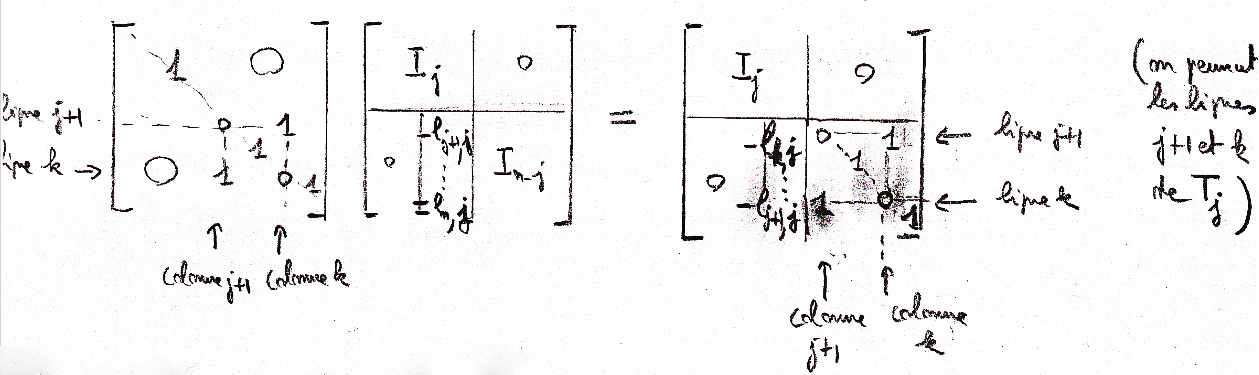
\includegraphics[scale=0.33]{matrices1.png}
\end{figure}

Cela revient au même de faire d'abord la permutation des lignes de $A^{(j-1)}$ puis la
combinaison linéaire où l'on permute les coefficients $l_{k,j}$ et $l_{j+1,j}$ (cf la
propriété de $P$ donnée plus loin : on permute les colonnes $j+1$ et $k$ de $T_j$).
\begin{figure}[h]
    \centering
    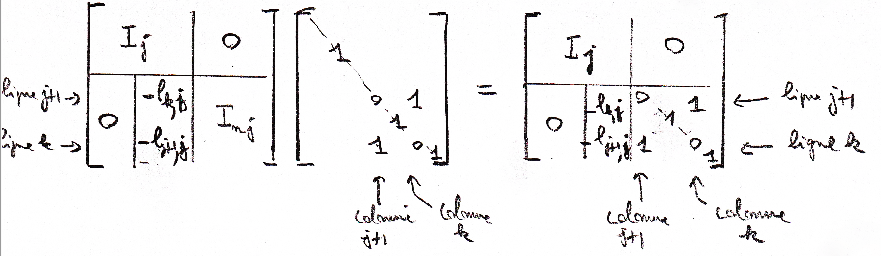
\includegraphics[scale=0.45]{matrices2.png}
\end{figure}

Donc les coefficients $l_{ij}$ du théorème 1 (coefficients de l'élimination de Gauss faite
sous permutation sur $PA$) s'obtiennent par permutation des coefficients $l_{ij}$ du
paragraphe 1) correspondant à l'élimination de Gauss sur la matrice $A$.
\end{remark}



\section{Techiques de choix du pivot}

Le choix d'un pivot non nul mais très petit peut conduire à des erreurs numériques importantes.
Par exemple, le système :
\begin{equation*}
    \left\lbrace
    \begin{array}{c}
        \varepsilon \; x_1 + x_2 = 1 \\
        x_1 + x_2 = 0 
    \end{array} \right.
\end{equation*}
a pour $\varepsilon \ne 1$ une solution unique $x_1 = -x_2 = \displaystyle\frac{1}{\varepsilon - 1}$

\begin{enumerate}[label=-]
    \item Si on résout (\ref{eq:S}) par la méthode de Gauss en utilisant $\varepsilon$ comme
        pivot, on obtient le système équivalent :
            \begin{align}
                \label{eqpivot1}
                \varepsilon \; x_1 = \; & 1 - x_2  \\
                x_2 (\frac{1}{\varepsilon} - 1) = \; & \frac{1}{\varepsilon} 
                \label{eqpivot2}
            \end{align}
\end{enumerate}

Par exemple , fixons $\varepsilon = 10^{-6}$. On simule un calcul
en virgule flottante avec 5 chiffres significatifs. Alors
$\frac{1}{\varepsilon} = 0,1.10^{7}$ (valeur exacte : $0,999999.10^6$)
d'où $x_2 = 1$ (valeur exacte : $x_2 = 10 \times \frac{100000}{999999} = 1,000001000001\dots$).

Mais alors $x_1 = 0$, ce qui est complètement faux (valeur exacte :
$x_1 = -x_2$).

Dans le membre de droite de (\ref{eqpivot1}), on effectue une 
soustraction qui est très mal conditionnée car $x_2 \approx 1$. Dans le calcul à
virgule flottante, on a $1 - x_2 = 0$, alors que la valeur exacte est 
$1 - x_2 \approx - 10^6$; on commet donc une erreur relative de $100 \%$,
alors que $x_2$ est connu avec une erreur relative de $10^{-6}$.

Si on choisit 1 comme pivot, on obtient :

\begin{equation*}
     \left \lbrace
     \begin{array}{ccc}
         x_1 + x_2  = & 0 \\[7pt]
         (1 - \varepsilon) x_2  = & 1
     \end{array}
     \right.
\end{equation*}

Alors $-\varepsilon + 1 = +0,1.10^1$ en virgule flottante (valeur exacte
$+0,999999$ d'où $x_2 = +1$ (précision $\sim 10^{-6}$) et $x_1 = -1$ (précision
$\sim 10^{-6}$).

Cela motive la :

\subsection*{Méthode de Gauss avec pivot partiel}
Même lorsque $a_{11} \ne 0$, on permute la 1\up{ère} ligne de (\ref{eq:S}) avec la
ligne où $|a_{i1}|$ est le plus grand. La même stratégie est répétée pour tous les
sous-systèmes apparaissant dans l'élimination de Gauss.

\begin{remark}
    Il existe aussi une méthode de Gauss avec pivot total, où on choisit comme
    pivot $a_{i_0,j_0}$ avec $|a_{i_0,j_0}| = \Max |a_{ij}|$.

    On permute alors la 1\up{ère} ligne de (\ref{eq:S}) avec la ligne $i_0$, et on
    permute les inconnues $x_1$ et $x_{j_0}$. On répète ce procédé pour tous
    les sous-systèmes qui apparaissent ensuite dans l'élimination de Gauss.

    La méthode avec pivot partiel est la plus employée. Elle marche bien en pratique.
    La méthode avec pivot total est plus coûteuse en temps de calcul; elle est donc
    assez peu employée.
\end{remark}


\section{Le coût de la méthode de Gauss}

\begin{eqnarray}
    \begin{split}
        Ax = b & \Leftrightarrow & PAX = Pb \\
        & \Leftrightarrow & LUX = Pb
    \end{split}
    \label{S1}
\end{eqnarray}

Résoudre \ref{S1} en 3 étapes :
\begin{enumerate}
    \item Factoriser $A$ ($PA = LU$)
    \item Résoudre $LC = Pb$ (méthode de remontée)
    \item Résoudre $UX = c$ (méthode de descente)
\end{enumerate}

\vspace{1cm}
\begin{remark}
    \begin{enumerate}
        \item L'étape 1. est la plus coûteuse
        \item Utiliser Fact-LU quand on a plusieurs systèmes linéaires. Avec la même matrice à résoudre : $AX^{(i)}=b^{(i)}, \; i = 1,2 \dots$
    \end{enumerate}
\end{remark}

\vspace{1cm}

* Factorisation $A=LU \; \; \; (P=I)$, à l'étape 1 de la factorisation : passage $A \to A^{(2)}$

\begin{enumerate}
    \item $(n-1)$ divisions (calcul de $l_{21}, \dots, l_{n1}$
    \item $2n(n-1)$ multitplications et additions (calcul $a_{ij}-l_{i1}a_{1j}, 2 \leq i \leq n, 1 \leq j \leq n$
    \item Passage $b$ à $b^{(2)}$, $2(n-1)$ multiplications et additions ($b_i - l_{i1}b_{1}, 2 \leq i \leq n$
\end{enumerate}

Il faut renouveler cette procédure pour les sous-systèmes de taille $n-1,n-2,\dots,2$

\underline{Au total}

\begin{equation*}
    \begin{rcases}
        \sim 2 \sum_{i=1}^n (n-i)^2 = 2.\frac{1}{3}n (n-\frac{1}{2})(n-1) \hspace{2cm}& +, *\\
        \sim 3 \sum_{i=1}^n (n-i) = 3.\frac{1}{2}n(n-1) \hspace{2cm} & +,*,\div
    \end{rcases}
    \text{$\Rightarrow \frac{2}{3}n^3+O(n^2)$}
\end{equation*}

* Réoslution d'un système triangulaire (étape de remontée)
(schéma pas pris)
\[
    X_n = \frac{b_n}{U_{nn}}
    x_i = \frac{1}{U_{2i}}(b_i - \sum_{k=i+1}^n a_{iK}X_K
\]

\begin{equation*}
    \text{$O(n^2)$}
    \begin{lcases}
        1 + 2 + 3 + \dots + n - 1 & = & \sum_{i=1}^{n-1}i = \frac{1}{2}(n-1)(n-2)\\
        1 + 2 + 3 + \dots + n - 1 & = & \sum_{i=1}^{n-1}i = \frac{1}{2}(n-1)(n-2)\\
        \text{n divisions}
    \end{lcases}
\end{equation*}

$\Rightarrow$ Donc la méthode de Gauss nécessite $\frac{2}{3}n^3+O(n^2)$ opérations.

\vspace{0.5cm}
\begin{remark}
    \begin{enumerate}
        \item Le pivot partiel a un coût en $O(n^2)$.
            \begin{itemize}
                \item [$\rightarrow$] Trouver le max parmi $n,n-1, \dots, 2, 1$ coeff.
            \end{itemize}

        \item Le pivot toal a un coût en $O(n^3)$
            \begin{itemize}
                \item [$\rightarrow$] Trouver le max parmi $n^2, (n-1)^2, \dots , 2^2, 1^2$ coeff.
            \end{itemize}
    \end{enumerate}
\end{remark}





